\documentclass[11pt]{amsart}
\usepackage{geometry}                % See geometry.pdf to learn the layout options. There are lots.
\geometry{letterpaper}                   % ... or a4paper or a5paper or ... 
%\geometry{landscape}                % Activate for for rotated page geometry
%\usepackage[parfill]{parskip}    % Activate to begin paragraphs with an empty line rather than an indent
\usepackage{graphicx}
\usepackage{subfigure}
\usepackage{amssymb}
\usepackage{epstopdf}
\DeclareGraphicsRule{.tif}{png}{.png}{`convert #1 `dirname #1`/`basename #1 .tif`.png}

\newenvironment{packed_enum}{
\begin{enumerate}
  \setlength{\itemsep}{1pt}
  \setlength{\parskip}{0pt}
  \setlength{\parsep}{0pt}
}{\end{enumerate}}

\title{Graph Theory Worksheet}
\author{Math 300}
%\date{}                                           % Activate to display a given date or no date

\begin{document}
\maketitle
%\section{x}
%\subsection{}



{\bf Radio Frequency Allocation}
Consider the following table of distances between radio stations labeled 1-6. For each station, 1 through 6, create an edge by drawing a line between the stations if the distance between the two is 150 or less.  What is the smallest number of colors needed to give each of the numbered dots (verticies) of this graph a color so adjacent vertices (edge between them) have different colors?  How do you know this number is the smaller number of colors needed?

\begin{center}
 \begin{tabular}{c|c|c|c|c|c|c} 
 \hline
  & 1	 & 2 & 3 & 4 & 5 & 6 \\
 \hline
 1 & - & 85 & 175 &200 & 50 & 100 \\ 
 \hline
 2 &  85 & - & 125 & 175 & 100 & 160 \\ 
 \hline
 3 & 175 & 125 & - &100 & 200 & 250 \\ 
 \hline
 4 & 200 & 175 & 100 & - & 210 & 220 \\ 
 \hline
 5 &  50 & 100 & 200 & 210 & - & 100 \\  
 \hline
  6&  100 & 160 & 250 & 220 & 100 & - \\ 
 \hline
\end{tabular}
\end{center}

  \begin{figure}[htp]
  \begin{center}
    \subfigure{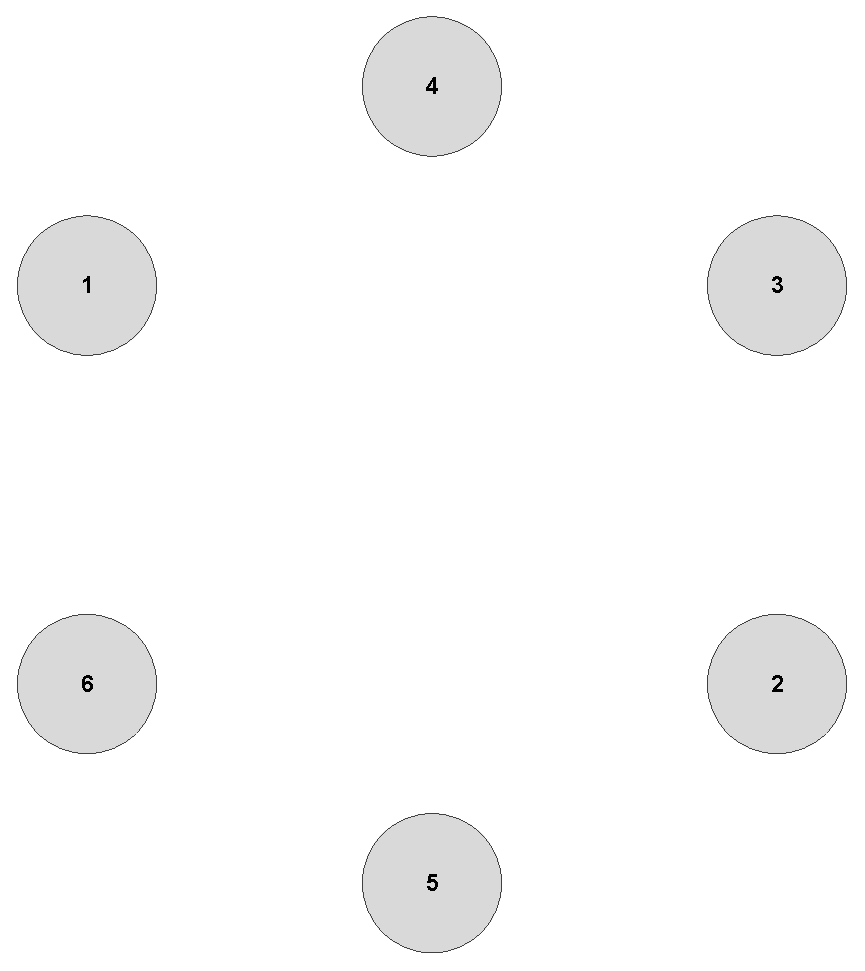
\includegraphics[scale=.50]{RFallocation1}}

    \end{center}
\end{figure}

\pagebreak

{\bf Puzzle of Alcuin} A traveler comes to a riverbank with a wolf, a goat, and a head of cabbage. To his delight he sees there a boat that he can use for crossing over to the other bank, but to his dismay, he notices that it can carry no more than two-the traveler himself, of course, and just one of the two animals or the cabbage. As the traveler knows, if left alone together, the goat will eat the cabbage and the wolf will eat the goat. The wolf does not eat cabbage. How does the traveler transport his animals and his cabbage to the other side intact in a minimum number of back-and-forth trips?

  \begin{figure}[htp]
  \begin{center}
    \subfigure{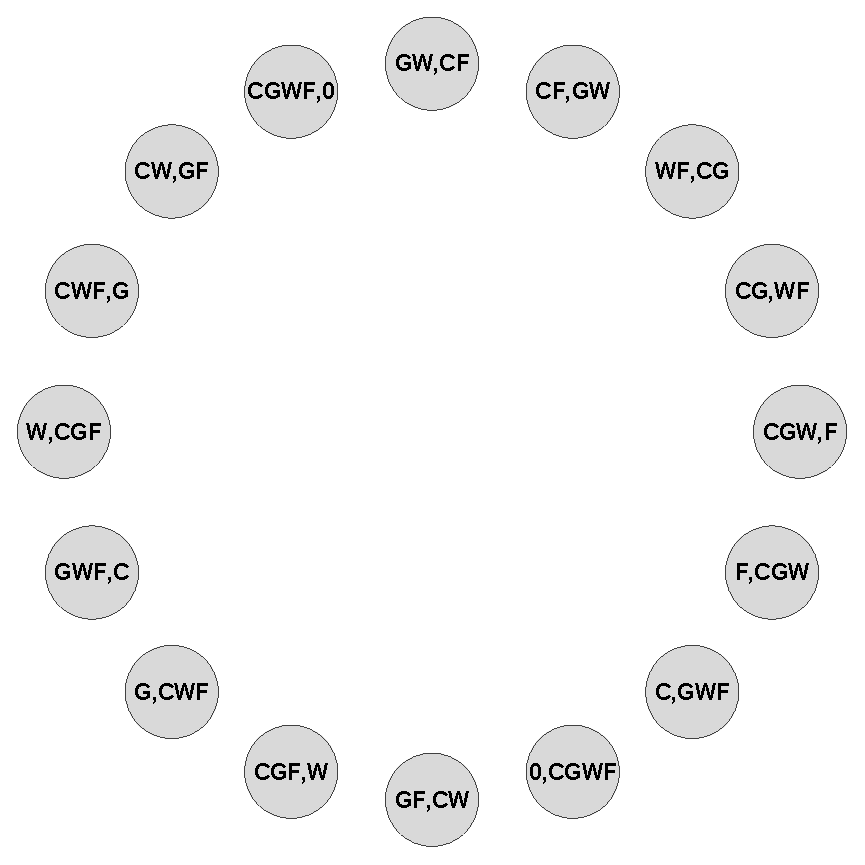
\includegraphics[scale=.50]{CGWFgraph1.pdf}}

    \end{center}
\end{figure}

{\bf Construct a graph} Consider all possible distributions of the Cabbage, Goat, Wolf, and Farmer on the two banks of a river.  They are listed above.  For example, (CG,WF) means that the cabbage and goat are on the left bank of the river and the wolf and farmer are on the right bank of the river.  Start out by X-ing out all of the bad (or impermissible) states like this one.  Then add lines between states if you can move between the states with one boat ride.  For example (CW, FG) and (CWF, G) should be connected because you can go from one state to the other by the Farmer riding across the river by himself.  Make lines to represent all such connections.




\end{document}  